% !TEX TS-program = pdflatex
% !TEX encoding = UTF-8 Unicode

\documentclass{beamer}
% for handouts: \documentclass[handout]{beamer}

%\setbeamertemplate{background canvas}[vertical shading][bottom=white,top=structure.fg!25]
% or whatever

\usetheme[compress]{Amsterdam}
%\setbeamertemplate{headline}{}
%\setbeamertemplate{footline}{}
%\setbeamersize{text margin left=0.5cm}
  
\usepackage[english]{babel}
\usepackage{listings}
\usepackage{geometry}
\usepackage{hyperref}

\usepackage{color}
\usepackage[T1]{fontenc}
\usepackage[utf8]{inputenc}
\usepackage{lmodern}

\usepackage{multicol}
\lstset{
basicstyle=\scriptsize\ttfamily,
columns=flexible,
breaklines=true,
numbers=left,
%stepsize=1,
numberstyle=\tiny,
backgroundcolor=\color[rgb]{0.85,0.90,1}
}


\begin{document}

\title[Big Data and Automated Content Analysis]{\textbf{Big Data and Automated Content Analysis\\ Part I+II} \\ Week 13 -- Wednesday \\ »Word Embeddings«}
\author[Damian Trilling]{Damian Trilling \\ ~ \\ \footnotesize{d.c.trilling@uva.nl \\@damian0604} \\ \url{www.damiantrilling.net}}
\date{8 May 2019}
\institute[UvA]{Afdeling Communicatiewetenschap \\Universiteit van Amsterdam}


\begin{frame}{}
\titlepage
\end{frame}

\begin{frame}{Today}
\tableofcontents
\end{frame}





%\begin{frame}[plain]
%\makebox[\linewidth]{
%	\includegraphics[width=\paperwidth,height=\paperheight,keepaspectratio]{../../pictures//topicscores}}
%\end{frame}


\section{From word counts to word vectors}

\begin{frame}[plain]
From word counts to word vectors
\end{frame}


\begin{frame}{Our BOW approach until now}
\begin{block}{Representing a document by word frequency counts}
Result of preprocessing and vectorizing:

0. \texttt{He took the dog for a walk to the dog playground}\\
$\Rightarrow$ \texttt{took dog walk dog playground}\\
$\Rightarrow$ \texttt{'took':1, 'dog': 2, walk: 1, playground: 1}
\end{block}

Consider these other sentences
\begin{enumerate}
	\item<2-> He took the doberman for a walk to the dog playground
	\item<3-> He took the cat for a walk to the dog playground
	\item<4-> He killed the dog on his walk to the dog playground 
\end{enumerate}

\onslide<5>{The vectorized representations of these sentences have a ``distance'' (dissimilarity) of 1 each, but arguably, sentences 0 and 1 should be ``closer'' than others}

\end{frame}


\begin{frame}{Our BOW approach until now}
\begin{itemize}
	\item Our vectorizers gave a random ID to each word
	\item What if we instead would represent each word by another vector representing its meaning?
	\item For, instance, `doberman' and `dog' should be represented by vectors that are close to each other in space, while `kill' and `walk' should be far from each other.
\end{itemize}
\pause
$\Rightarrow$ That's the idea behind word embeddings!

\pause

Or, more broadly: Can computers understand meanings, semantic relationships, different types of contexts?
\end{frame}


\section{Training word embeddings}
\begin{frame}[plain]
Training word embeddings
\end{frame}

\begin{frame}{Continous Bag of Words (CBOW) vs skipgram}
Example sentence: ``the quick brown fox jumped over the lazy dog''
\begin{block}{CBOW: Predict a word given its context}
Dataset:

\texttt{([the, brown], quick), ([quick, fox], brown), ([brown, jumped], fox), ...}
\end{block}

\pause


\begin{block}{skipgram: Predict the context given the word}	
\texttt{(quick, the), (quick, brown), (brown, quick), (brown, fox), ...}
\end{block}

\tiny{Example taken from here: \url{https://medium.com/explore-artificial-intelligence/word2vec-a-baby-step-in-deep-learning-but-a-giant-leap-towards-natural-language-processing-40fe4e8602ba}}
\end{frame}

%window sizes


\begin{frame}{Continous Bag of Words (CBOW) vs skipgram}
\begin{itemize}
	\item CBOW is faster
	\item skipgram works better for infrequent words
	\item Both are often used
	\item Usually, we use larger window sizes (e.g, 5)
	\item We need to specify the number of dimensions (typically 100--300)
\end{itemize}
\pause

\textit{In any event, as a result of the prediction task, we end up with a \{100|200|300\}-dimensional vector representation of each word.*}



\tiny{* If that makes you think of PCA/SVD, that's not completely crazy, see Levy, O., Goldberg, Y., \& Dagan, I. (2018). Improving Distributional Similarity with Lessons Learned from Word Embeddings. \textit{Transactions of the Association for Computational Linguistics, 3}, 211--225. doi:10.1162/tacl\_a\_00134}\\
\end{frame}


\begin{frame}{``...a word is characterized by the company it keeps...'' (Firth, 1957)}
\begin{block}{Word embeddings \ldots}
	\begin{itemize}
		\item help capturing the meaning of text
		\item are low-dimensional vector representations that capture semantic meaning
		\item are state-of-the-art in NLP...
	\end{itemize}
\end{block}

\tiny{Firth, J. R. (1957). A synopsis of linguistic theory, 1930-1955. Studies in linguistic analysis.}
\end{frame}

%Due to developments in the field of NLP, algorithms have become increasingly apt to understand human language. Word embeddings are the current state of the art for capturing the meaning of texts. Word embeddings are vector representations of words. They are the current state of the art in NLP to understand, capture and process language. The basic idea of word embeddings is that one gets to know a word by looking at the company that it keeps; contexts is crucial in understanding word meaning. 


\begin{frame}{You can literally calculate with words!}
And answer questions such as ``Man is to woman as king is to \_\_\_\_?''
\makebox[\linewidth]{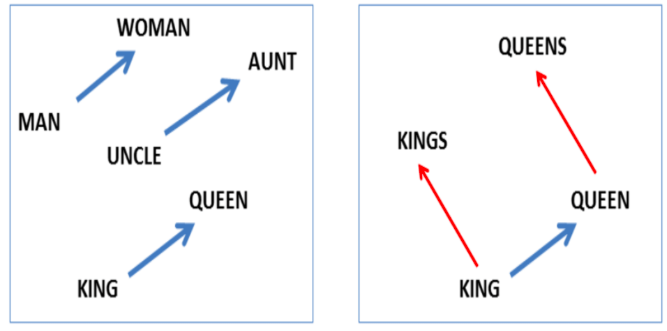
\includegraphics[width=\linewidth,height=\textheight, keepaspectratio]{../../pictures/embeddings.png}}
semantic relationships vs. syntactic relationships
\end{frame}

%word vectors that are able to capture the relationships between words in a surprisingly expressive way. Word embeddings are especially effective in understanding analogies, and for example understand that man is to woman as uncle to aunt, and king to king. 



\section[Improving models]{Using word embeddings to improve models}
\begin{frame}[plain]
Using word embeddings to improve models
\end{frame}

\begin{frame}{In supervised machine learning}
\begin{itemize}[<+->]
	\item Modify CountVectorizer or TfIdfVector such that for each term, you do not only count how often it occurs, but also multiply with its embedding vector
	\item Often, pre-trained embeddings (e.g., trained on the whole wikipedia) are used
	\item Thus, our supervised model will be able to deal with synonyms and related words!
\end{itemize}

\pause 
Let's look at an example for using supervised sentiment analysis (i.e., what we did with IMDB-data before).


\end{frame}



\begin{frame}[plain]
\makebox[\linewidth]{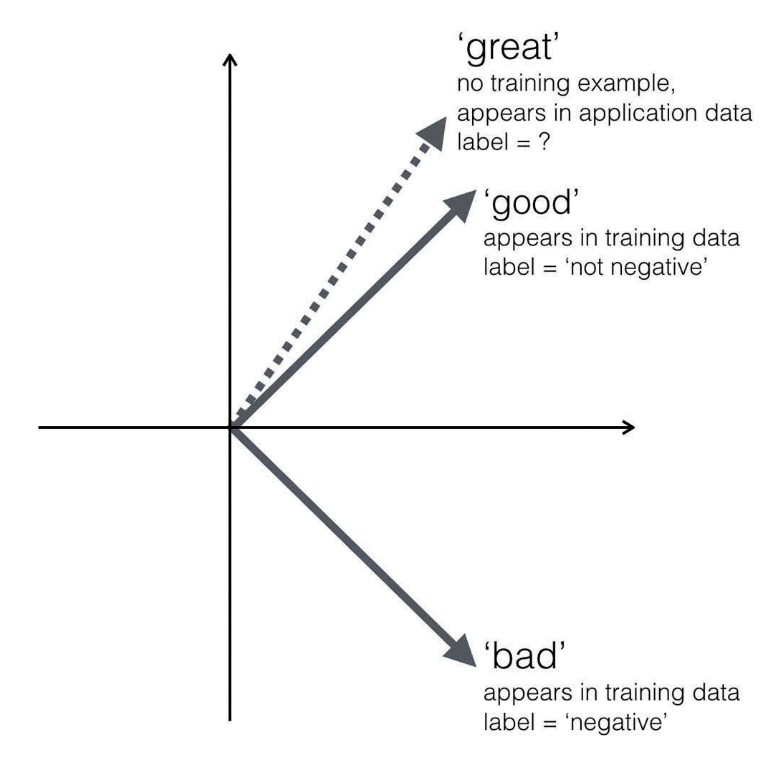
\includegraphics[width=\linewidth,height=\textheight, keepaspectratio]{../../pictures/rudkowsky2018-1}}

\tiny{Rudkowsky, E., Haselmayer, M., Wastian, M., Jenny, M., Emrich, Š., \& Sedlmair, M. (2018). More than Bags of Words: Sentiment Analysis with Word Embeddings. \textit{Communication Methods and Measures, 12}(2–3), 140–157. doi:10.1080/19312458.2018.1455817}
\end{frame}


\begin{frame}{It's not always black/white\ldots}
Sometimes, BOW may be just fine (for very negative sentences, it doesn't matter). But especially in less clear cases ('slightly negative'), embeddings increased performance.
\makebox[\linewidth]{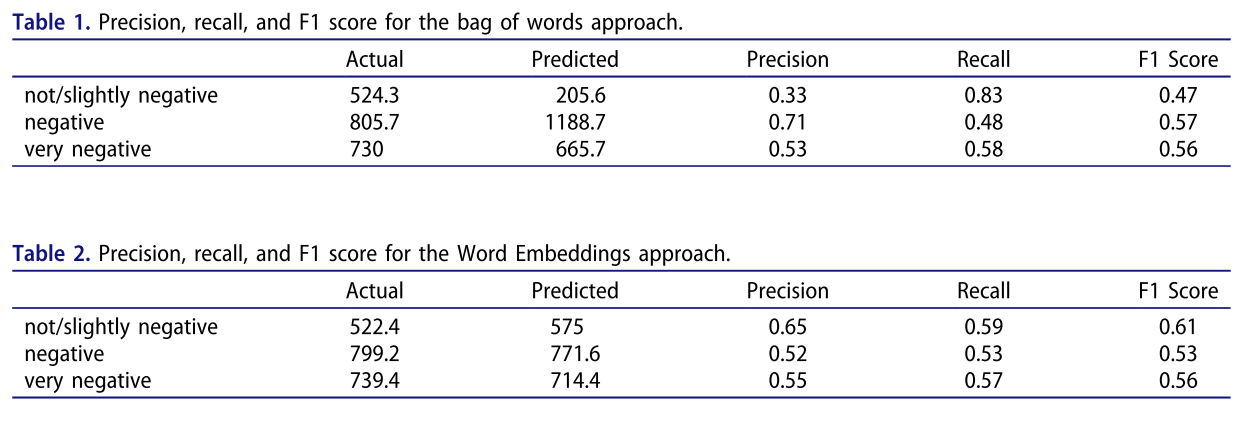
\includegraphics[width=\linewidth,height=\textheight, keepaspectratio]{../../pictures/rudkowsky2018-2}}

\vfill

\tiny{Rudkowsky, E., Haselmayer, M., Wastian, M., Jenny, M., Emrich, Š., \& Sedlmair, M. (2018). More than Bags of Words: Sentiment Analysis with Word Embeddings. \textit{Communication Methods and Measures, 12}(2–3), 140–157. doi:10.1080/19312458.2018.1455817}
\end{frame}



\begin{frame}{In document similarity calculation}
\begin{block}{Use cases}
	\begin{itemize}
	\item plagiarism detection
	\item Are press releases/news agency copy/\ldots taken over?
	\item Event detection
	\end{itemize}
\end{block}
\pause
\begin{block}{Traditional measures}
	\begin{itemize}
		\item Levenshtein distance (How many characters|words do I need to change to transform string A into string B?)
		\item Cosine similarity (``correlation'' between the BOW-representations of string A and string B)
	\end{itemize}
\end{block}
\end{frame}


\begin{frame}[plain]
BUT: This only works for literal overlap. What if the writer chooses synonyms?
\pause 

\makebox[\linewidth]{\includegraphics[width=\linewidth,height=\textheight, keepaspectratio]{../../pictures/wmd}}


\tiny{Kusner, M. J., Sun, Y., Kolkin, N. I., \& Weinberger, K. Q. (2015). From Word Embeddings To Document Distances. \textit{Proceedings of The 32nd International Conference on Machine Learning} (Vol. 37, pp. 957–966)}
\end{frame}


\begin{frame}{There are several approaches}
\begin{itemize}
	\item word mover's distance
	\item soft cosine similarity
\end{itemize}
In common: we use pre-trained embeddings to replace words (that otherwise would just have a random identifier and be unrelated) with vectors representing their meaning, when calculating our measure of interest
\end{frame}


\section[Detecting biases]{(Ab-)using word embeddings to detect biases}
\begin{frame}[plain]
(Ab-)using word embeddings to detect biases
\end{frame}

\begin{frame}{Biased embeddings}
\begin{itemize}
	\item word embeddings are trained on large corpora
	\item As the task is to learn how to predict a word from its context (CBOW) or vice versa (skip-gram), biased texts produce biased embeddings
	\item If in the training corpus, the words ``man'' and ``computer programmer'' are used in the same context, then we will learn such a gender bias
\end{itemize}

\tiny{Bolukbasi, T., Chang, K.-W., Zou, J., Saligrama, V., \& Kalai, A. (2016). Man is to Computer Programmer as Woman is to Homemaker? Debiasing Word Embeddings, 1–25. Retrieved from http://arxiv.org/abs/1607.06520}
\end{frame}


\begin{frame}{Biased embeddings}
Usually, we do not want that (and it has a huge potential for a shitstorm)

~\\
\pause

unless\ldots

~\\
\pause

we actually want to chart such biases.

\end{frame}


\begin{frame}{An exmaple from our research}
We trained word embeddings on 3.3 million Dutch news articles.

Are vector representations of outgroups (Maroccans, Muslims) closer to representations of negative stereotype words than ingroups?
\vspace{.5cm}

\tiny{Kroon, A.C., Van der Meer, G.L.A., Jonkman, J.G.F., \&Trilling, D. (manuscript in prepration): Guilty by Association: Using Word Embeddings to Measure Ethnic Stereotypes in News Coverage}
\end{frame}


\begin{frame}[plain]
\makebox[\linewidth]{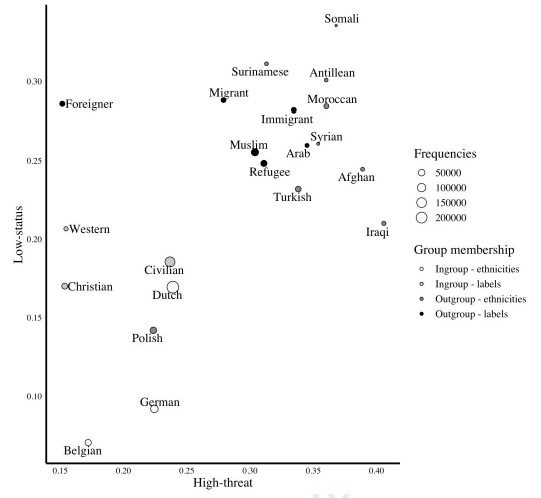
\includegraphics[width=\linewidth,height=\textheight, keepaspectratio]{../../pictures/embeddingbias}}

\end{frame}


\section[AEM]{AEM: An application from our own research}

\begin{frame}[plain]
We can use pre-trained embeddings -- but can we make even better ones?
\textbf{The Amsterdam Embedding Model (AEM)}\\


\vspace{1cm}

{\footnotesize{Anne Kroon, Antske Fokkens, Damian Trilling, Felicia Loecherbach, Judith Moeller, Mariken A. C. G. van der Velden, Wouter van Atteveldt} }
\end{frame}



%For all these tasks, you need to process text. 
%Humans are obviously very good in this. However, we are not capable of handling %humongous amounts of data. Therefore, we need computers. 
%For computers, it used to be relatively hard to understand language, to capture %semantic relations, especially in different type of contexts. 


\begin{frame}{Why do this?}
\begin{itemize}
\item Embedding models are of great interest to communication scholars
\item yet... Most publicly available models represent \textbf{English} language
\item The preparation of good-performing embedding models require a significant amount of \textbf{time} and \textbf{access to a large amount of data sets}
\item Few Dutch embedding models are available, but trained on ordinary human language from the World Wide Web.
\item These models do not capture the specifics of news article data and are therefore less suitable to study and understand dynamics of this domain
\item $\Rightarrow$ No model is available trained on Dutch news data
\end{itemize}
\end{frame}

%Properly trained embedding models are of great interest to communication scholars, because they can help with diverse tasks, such as topic classification, automated sentiment analysis or bias detection. Yet – currently no model exist that is trained on media data – and therefore effectively deals with the particularities of news media data. 

%\subsection{The Amsterdam Embedding Model}
\begin{frame}{Project's Aim}
\begin{block}{Aim of the current project} 
\begin{enumerate}
\item Develop and evaluate a high-quality embedding model
\item Assess performance in downstream tasks of interest to Communication Science (such as topic classification of newspaper data).
\item Facilitate distribution and use of the model
\item Offer clear methodological recommendations for researchers interested using our Dutch embedding model
\end{enumerate}
\end{block}
\end{frame}

%Therefore, this project was set out to develop a good word embedding model trained on Dutch media data, and facilitate its distribution


%\subsection{Approach and Preliminary Results}

\begin{frame}{Training data}
\begin{block}{Training data set}
\begin{itemize}
\item Dataset: diverse print and online news sources
\item Preprocessing: duplicate sentences were removed
\item Telegraaf (print \& online), NRC Handelsblad (print \& online), Volkskrant (print \& online), Algemeen Dabldad (print \& online), Trouw (print \& online), nu.nl , nos.nl
\item \# words: 1.18b (1181701742)
\item \# sentences: 77.1M (77151321)
\end{itemize}
\end{block}
\end{frame}

\begin{frame}{Training model}
\begin{block}{Training model}
\begin{itemize}
\item We trained the model using Gensim's Word2Vec package in Python
\item Skip-gram with negative sampling, window size of 5, 300-dimensional word vectors
\end{itemize}
\end{block}
\end{frame}

%\subsection{Evaluation}
\begin{frame}{Evaluation}
Evaluation of the Amsterdam Embedding Model
\end{frame}

\begin{frame}{Evaluation}
\begin{block}{Evaluation methods}
\begin{itemize}
\item To evaluate the model, we compare it to two other publicly available embedding models
\begin{itemize}
\item $\Rightarrow$ \textbf {'Wiki'}: Embedding model trained on Wikipedia data (FastText)
\item $\Rightarrow$ \textbf{'Cow'}: Embedding model trained on diverse .nl and .be sites (Schafer \& Bildhauer, 2012; Tulkens et al., 2016)
\item $\Rightarrow$ \textbf{'AEM'}: Amsterdam Embedding Model
\end{itemize}
\end{itemize}
\end{block}
\end{frame}

%To evaluate our model, we will compare it (at least in a first step) – to two other, publicly available word embedding models: One trained on Wikipedia data, and the other on divers dutch and Belgian websites. 

\begin{frame}{Evaluation data}
\begin{block}{Evaluation data}
\begin{enumerate}
\item 'relationship'/ analogy-task (Tulkens et al., 2016)
\begin{itemize}
\item \textbf{syntatic relationships}: dans dansen loop \textit{[lopen]}
\item \textbf{semantic relationships}: denemarken kopenhagen noorwegen \textit{[oslo]}
\end{itemize}
\item 5806 relationship tasks
\end{enumerate}
\end{block}
\end{frame}

%Tulkens et al created several Dutch relationship tasks. For example, when given dans (dance) dansen (dancing) and loop (walk), the computer has to guess that the word we are looking for is lopen (walking). This is an example of syntactic analogy. The same applies to capital - country relations (Copenhagen is to Denmark as … [Oslo] to Norway]. This is an example of a semantic analogy. 
%Each model had to solve over 5K of these types of analogy tasks. We subsequently use these results to compare how well they do.

\begin{frame}{}
\makebox[\linewidth]{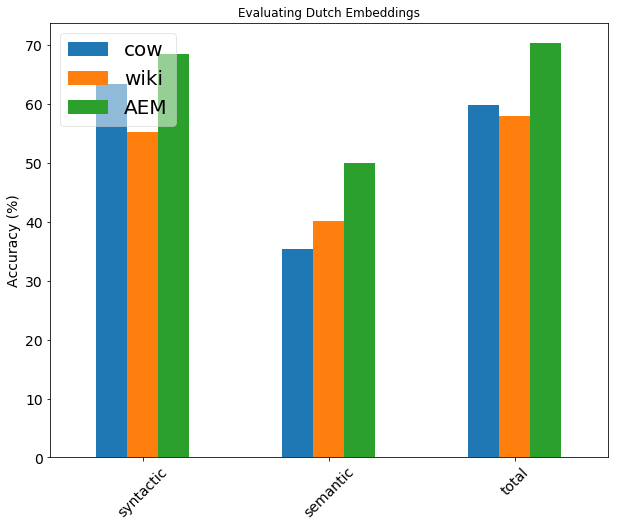
\includegraphics[width=\linewidth,height=\textheight, keepaspectratio]{../../pictures/evaluation_data.png}}
\end{frame}

%As can be seen, the AEM (= Amsterdam Embedding Model) outperfoms the other models on both syntactic analogies and semantic analogies. 

%\subsection{Illustration}
\begin{frame}{Illustration}
Illustration - Using the Amsterdam Embedding Model
\end{frame}

%Let's see what the model has learned about Dutch language. Now, we will provide some illustrations of how well the AEM understands the Dutch language. More specifically, we will provide a 2 dimensional visualisation of some random Dutch words in the word vector space..


\subsection{}
\begin{frame}{}
\makebox[\linewidth]{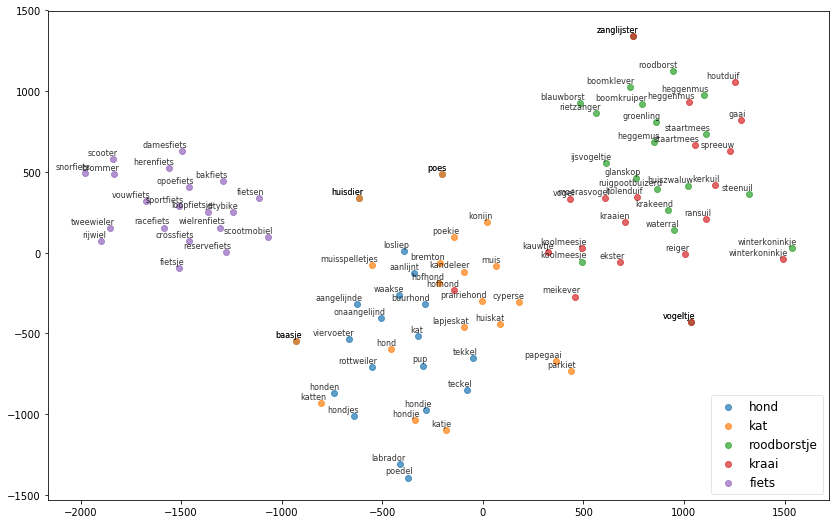
\includegraphics[width=\linewidth,height=\textheight, keepaspectratio]{../../pictures/w2v_300_illustration.png}}
\end{frame}

% this is a 2 dimensional representation of the most similar words to fiets, hond, kat, roodborstje and kraai 

\begin{frame}{}
\makebox[\linewidth]{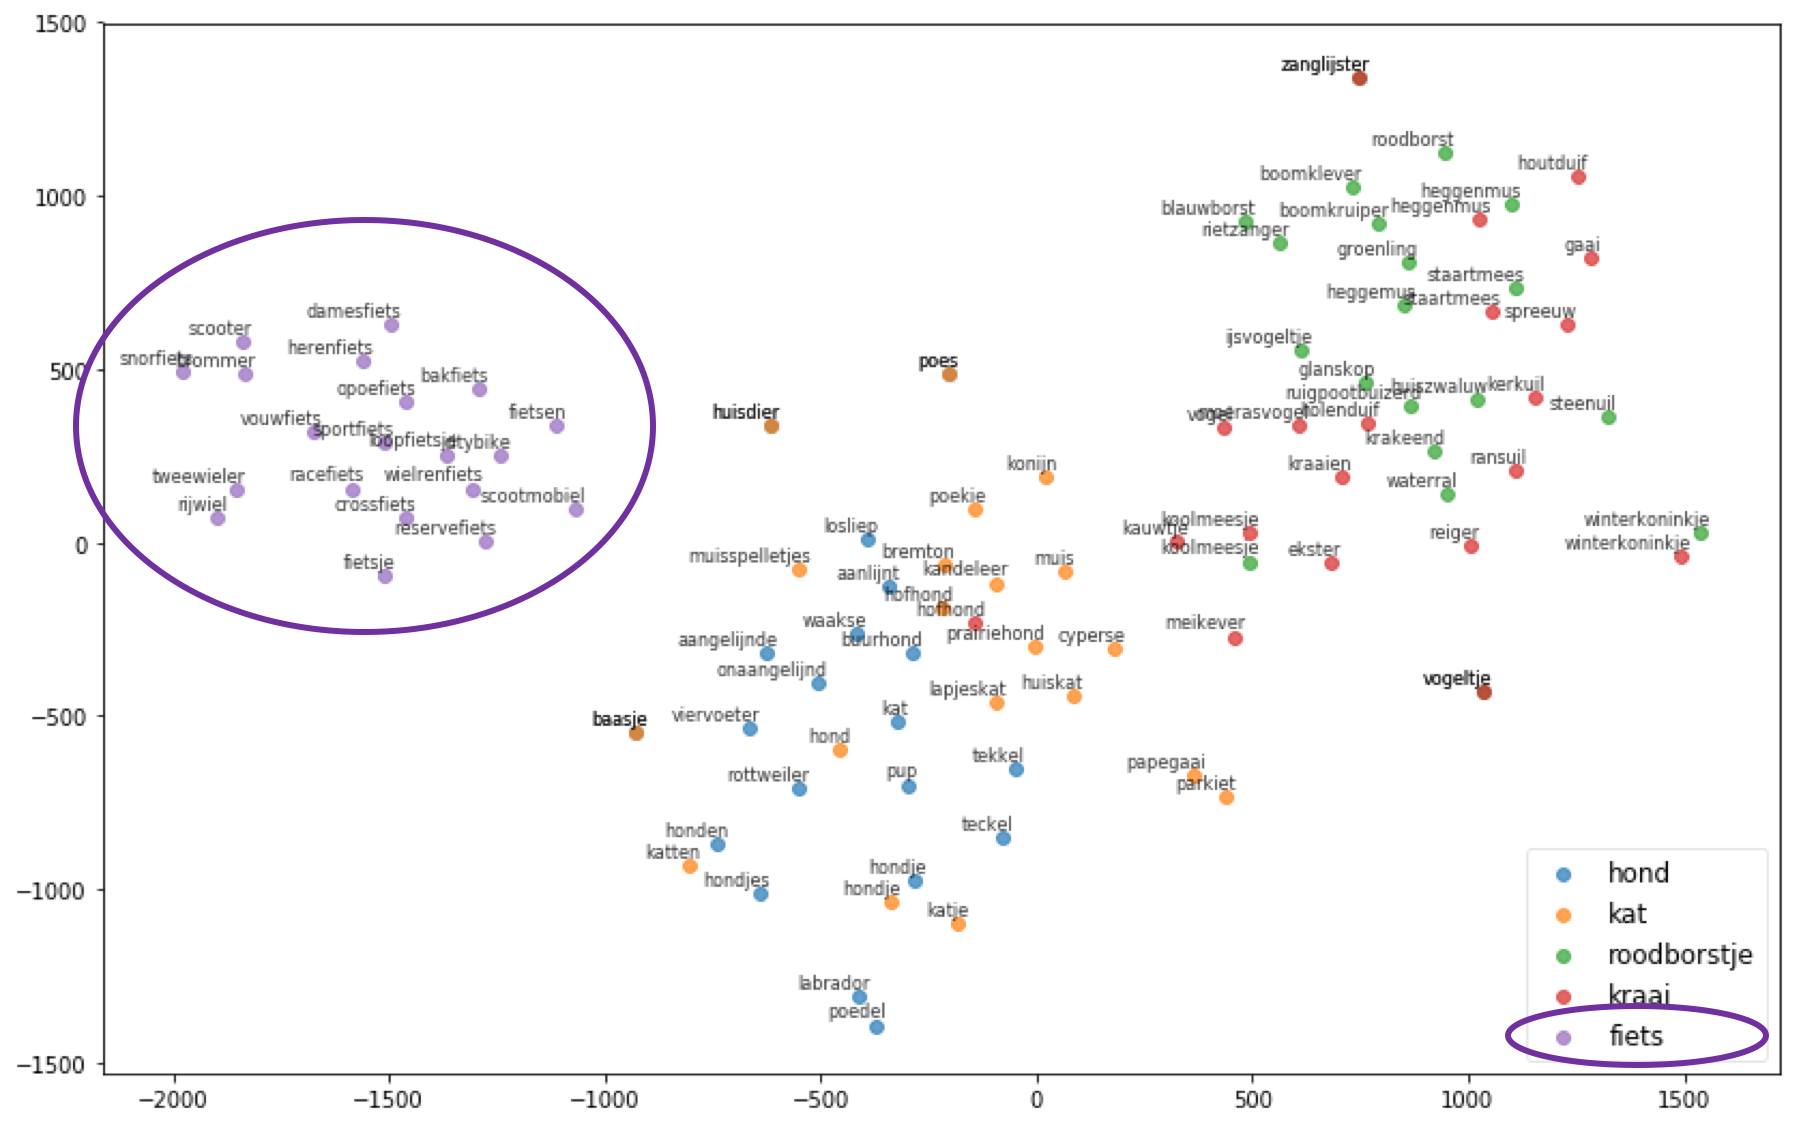
\includegraphics[width=\linewidth,height=\textheight, keepaspectratio]{../../pictures/visual2.png}}
\end{frame}

%as can be seen, words most similar to fiets are on the left. 

\begin{frame}{}
\makebox[\linewidth]{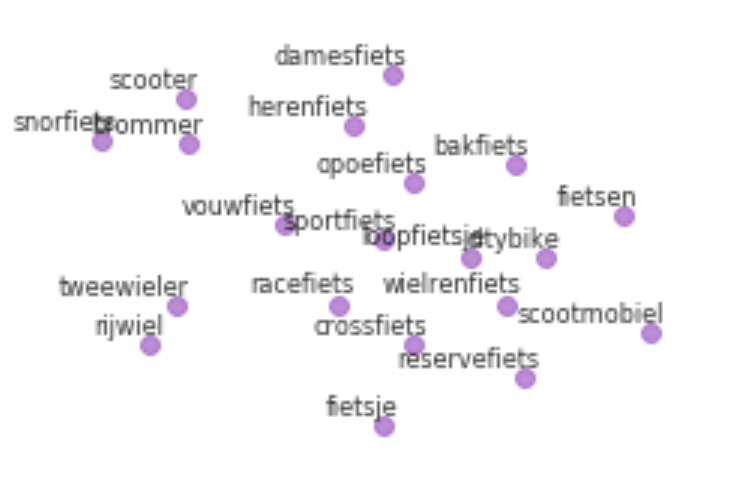
\includegraphics[width=\linewidth,height=\textheight, keepaspectratio]{../../pictures/fiets}}
\end{frame}

%the model has learned that fiets is similar to racefiets, wielrenfiets, rijwiel - and different from the animal department: it doesnt overlap with our kats/ dogs and birds clusters

\begin{frame}{}
\makebox[\linewidth]{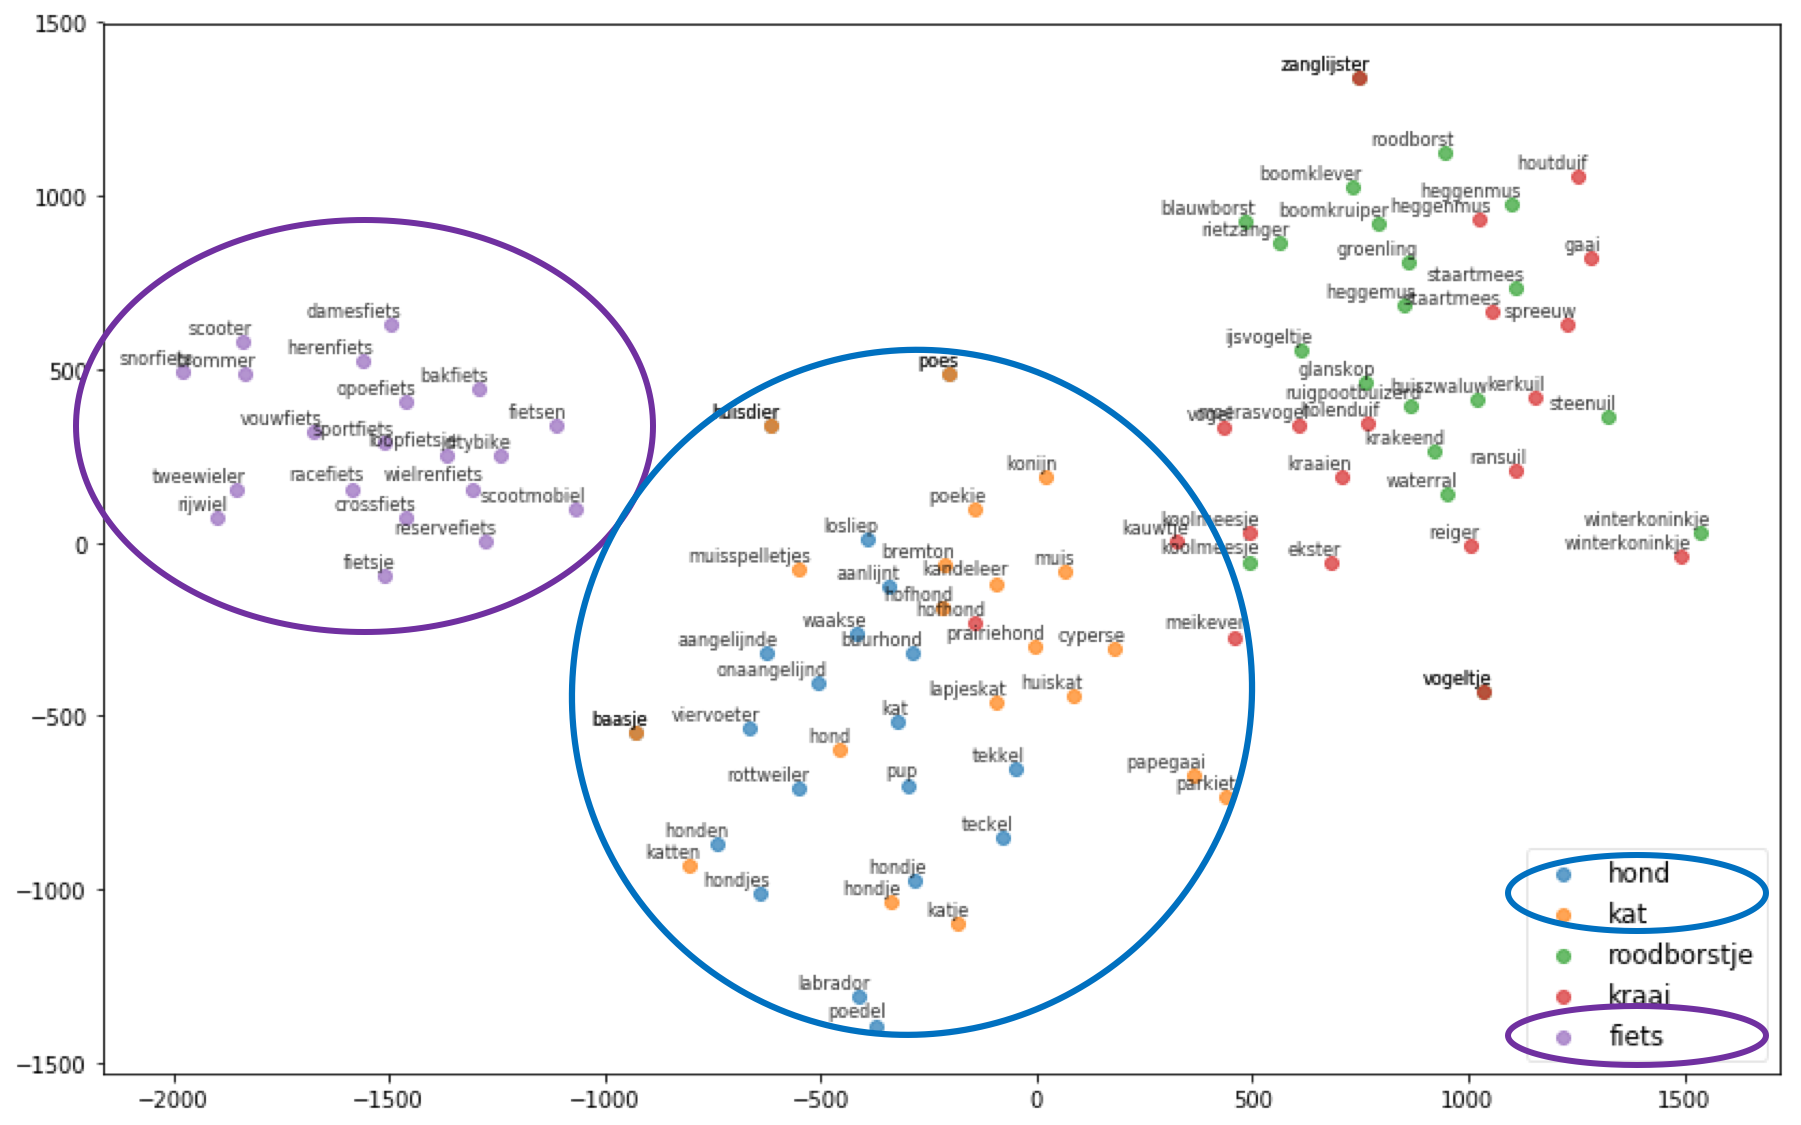
\includegraphics[width=\linewidth,height=\textheight, keepaspectratio]{../../pictures/visual1.png}}
\end{frame}

%the model recognizes that fiets is something else from honden and katten. Both mammals and pets, dogs and cats are quite similar and appear in the same cluster.  

\begin{frame}{}
\makebox[\linewidth]{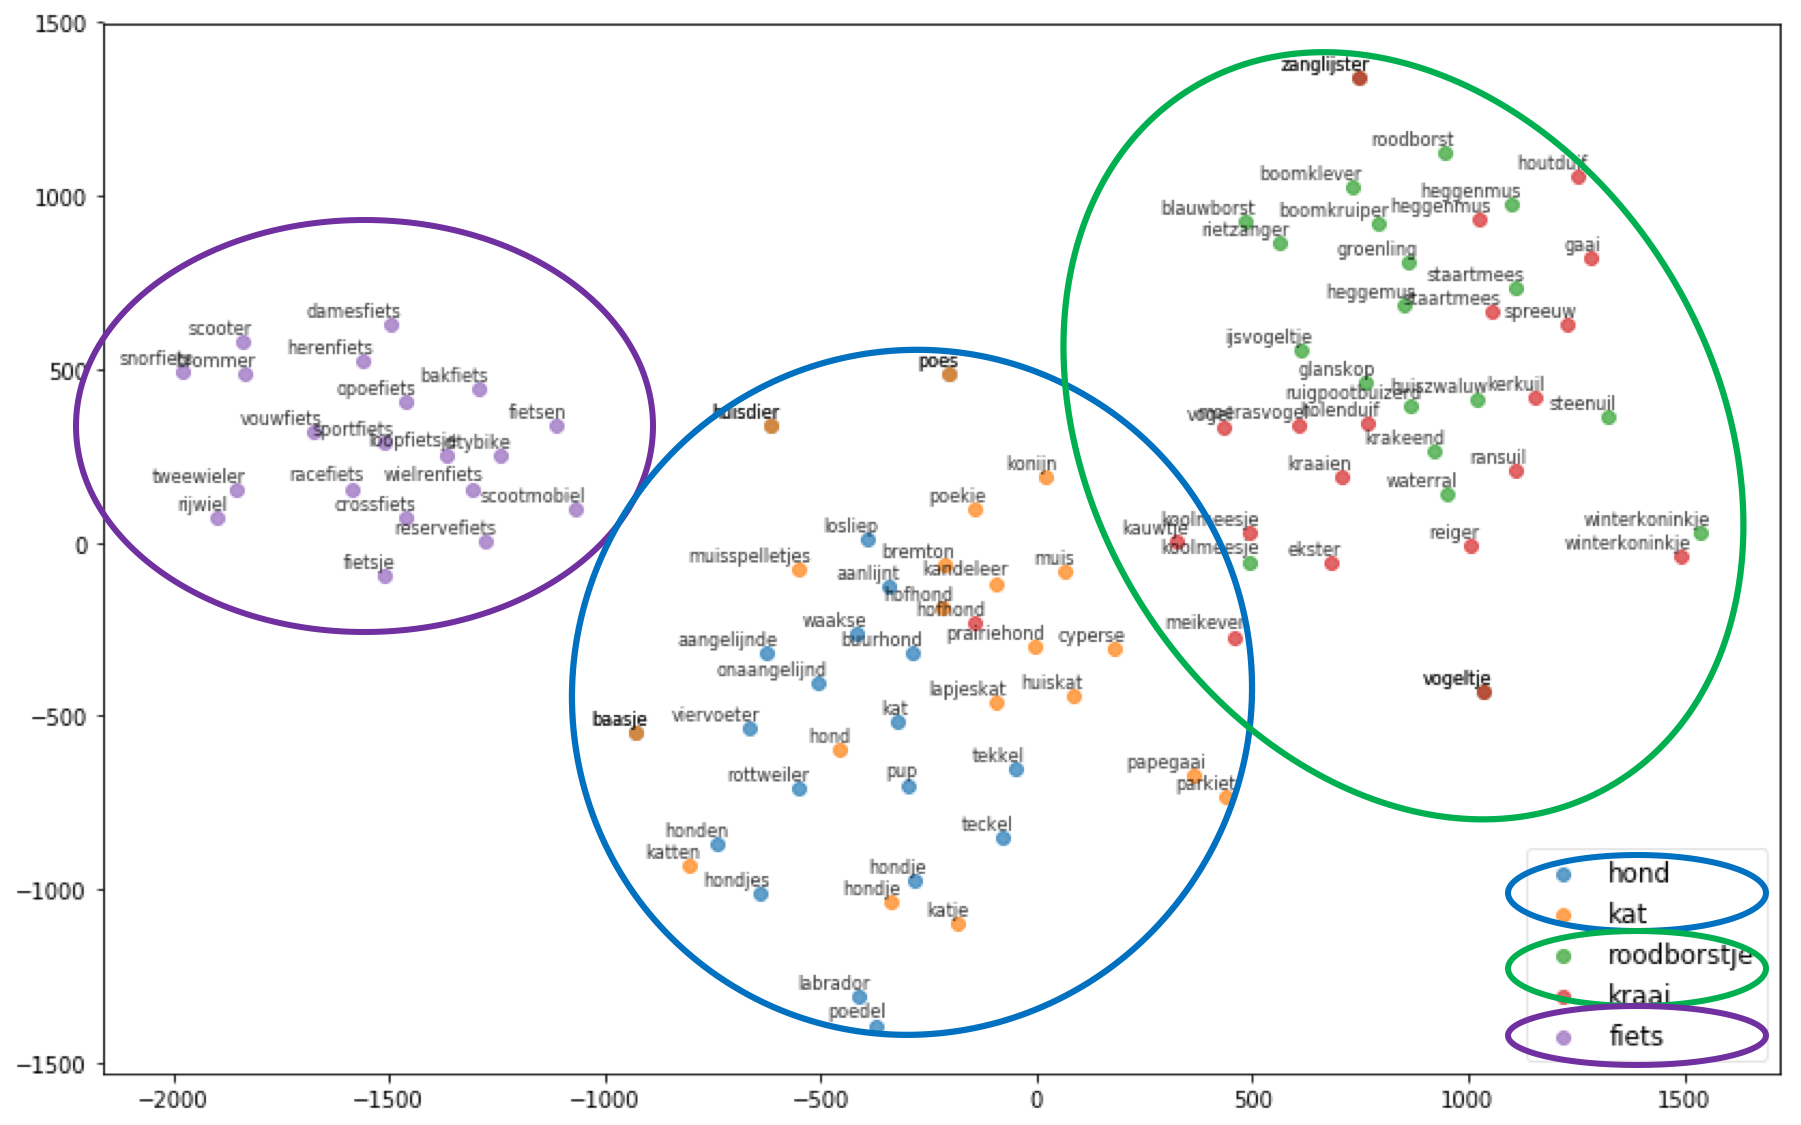
\includegraphics[width=\linewidth,height=\textheight, keepaspectratio]{../../pictures/visual.png}}
\end{frame}

%Finally, the model recognizes that dogs and kats are different from redbreasts and crows, with both appear in a 'bird-related' cluster.

%\begin{frame}{}
%	\makebox[\linewidth]{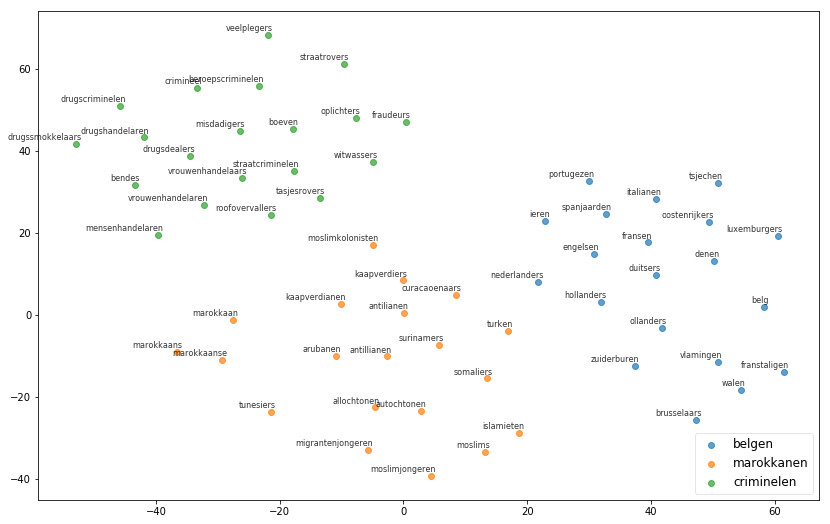
\includegraphics[width=\linew%idth,height=\textheight, %keepaspectratio]{../../pictures/bias.png}}
%\end{frame}

%Now we know that the model understands Dutch pretty well. We can now apply to model to diverse tasks that are of greater interest to communication scholars. For example, we can see whether or not our training data contains bias.When we plot the most similar words to ‘criminals, Belgians and Moroccans,  we see that Moroccans are much closer to criminals, that Belgians. THis could potentiall reveal bias in the training data.

%\subsection{Re-usability}
\begin{frame}{Re-usability}
Re-usability of the Amsterdam Embedding Model
\end{frame}

%\subsection{Availability of model and code}
\begin{frame}{Re-usability}
\begin{block}{Reusing model and data}
\begin{enumerate}
\item The final Amsterdam Embedding Model will be made available at \url{https://github.com/annekroon/AEM}
\item Open access to all the code
\end{enumerate}
\end{block}
\end{frame}




\section{Next meetings}
\begin{frame}{Next meetings}

\begin{block}{Friday}
Working with word embeddings in gensim.
(Fun tutorial, if you want to: \url{https://www.kaggle.com/pierremegret/gensim-word2vec-tutorial})
\end{block}

\begin{block}{Wednesday: Wrapping up and moving on}
What did we not cover? What are future directions?
\end{block}


\end{frame}




\end{document}

